\documentclass[]{aiaa-tc}% insert '[draft]' option to show overfull boxes

% packages
\usepackage{amsfonts}
\usepackage{amsmath}
\usepackage{xcolor}
\usepackage[margin=1in]{geometry}
\usepackage{mathtools}
\usepackage{hyperref}
\usepackage{listings}
\usepackage{pdfpages}
\usepackage{tcolorbox}
\usepackage{wrapfig}
\usepackage{graphicx}

\graphicspath{{../figs}}

% set up the hyperlink theme
\hypersetup{
    colorlinks=true,
    linkcolor=blue,
    urlcolor=blue,
    pdfpagemode=FullScreen,
    citecolor=blue,
    allcolors=blue
}

\title{The Gaussian Plume Model Revisited: Evaluating performance against unsteady, turbulent simulation}


 \author{ Ted Balabanski\thanks{Virginia Tech, Charles E. Via Jr. Department of Civil and Environmental Engineering} }

 % Data used by 'handcarry' option if invoked
 \AIAApapernumber{YEAR-NUMBER}
 \AIAAconference{Conference Name, Date, and Location}
 \AIAAcopyright{\AIAAcopyrightD{YEAR}}

 % Define commands to assure consistent treatment throughout document
 \newcommand{\eqnref}[1]{(\ref{#1})}
 \newcommand{\class}[1]{\texttt{#1}}
 \newcommand{\package}[1]{\texttt{#1}}
 \newcommand{\file}[1]{\texttt{#1}}


 % helpful "debugging" command from stackoverflow. prints out big [FIX]
\newcommand{\X}{\color{red}\large\textbf{[FIX]}\color{black}\normalsize}
\newcommand{\pd}[2]{\frac{\partial #1}{\partial #2}}
\newcommand{\dd}[2]{\frac{d #1}{d #2}}
\newcommand{\unit}[1]{\, \mathrm{#1}}
\newcommand{\fix}[1]{\color{red} #1 \color{black}}

\begin{document}

\maketitle

\begin{tcolorbox}[colback=blue!4!white,colframe=blue,title=A note to the instructor]
Throughout this manuscript, I use \fix{red text} to provide commentary on what will change between this extended abstract and the final manuscript due at the end of the semester. Please be advised of this annotation.
\end{tcolorbox}

\begin{abstract}
  Air pollution is an issue of global consequence, where short-term spikes can give serious health issues. The Gaussian Plume Model (GPM) is a widely-utilized model of mean air pollutant transport, used to regulate pollution discharge. In this study, we evaluate the GPM against a turbulent dataset of neutrally-bouyant smoke particles. \fix{Results and Discussion summary to follow, once results are more mature}.
\end{abstract}

\section*{Nomenclature}

\begin{tabbing}
  XXXXX \= \kill% this line sets tab stop
  $u$ \> Velocity \\
  $C$ \> Concentration \\
  $I, J, K$ \> Stability factors in calculating the variance of the GPM \\
  $\sigma^2$ \> Variance \\
  $U_0$ \> Mean wind speed in the downwind direction, $x_1$ \\
  $U_{rms}$ \> Root mean-square windspeed \\
  \textit{Subscript}\\
  $1, 2, 3$ \> Typically, relating to the three Cartesian axes, e.g., $(x_1, x_2, x_3)$ \\
\end{tabbing}

\section{Introduction}

\fix{Add a few sentences on the health impacts of poor air quality and why air quality modeling is important}

The Gaussian Plume Model (GPM) \cite{sinha_application_2025} is a semi-empirical model of contaminant transport discharging from an elevated point-source. The GPM is integrated into several available air quality software, including the EPA's AERMOD \cite{cimorelli_aermod_2005} package. The GPM has been used to model regional-scale particulate matter concentration in Poland \cite{kawka_downscaling_2023}, wildfire pollution in Italy \cite{lotrecchiano_pollution_2020}, and industrial pollution from oil refineries in Iraq \cite{salih_air_2025}.

The essence of the GPM is that in a steady-state, mean-wind driven flow, neutrally-bouyant air quality pollutants will advect downwind ($x_1$) and disperse in the vertical and transverse directions. The concentration profile ($C$) in the transverse ($x_2$) and vertical ($x_3$) is modeled as a Gaussian distribution, i.e., $C(x_2, x_3) \sim \mathcal{N}(c_0, \sigma_2^2, \sigma_3^2)$, where $c_0$ is the mean concentration at per unit area. A schematic of the GPM concentration profile for a smokestack point-source (the cannonical application for the GPM) is provided in Figure \ref{fig:plume-schematic}

The closed form of the GPM requires the calculation of the variance of the Gaussian distributions in the longitudinal and transverse directions, given by

\begin{equation} \label{eq:gpm-variances}
  \begin{aligned}
    \sigma_2^2 (x_1) &= \exp^2 \left[ I_2 + J_2 \ln x_1 + K_2 \left( \ln x_1 \right)^2 \right] \\
    \sigma_3^2 (x_1) &= \exp^2 \left[ I_3 + J_3 \ln x_1 + K_3 \left( \ln x_1 \right)^2 \right]
  \end{aligned}
\end{equation}

where the $I$, $J$, and $K$ are empirically derived stability coefficients, corresponding to atmospheric stability classes. Using the variances calculated in \eqnref{eq:gpm-variances}, we calculate the concentration at any point downwind with

\begin{equation} \label{eq:gpm}
  C = \left[ \frac{J_0}{U_0} \right] \left[ \frac{1}{\sigma_2 \sqrt{2 \pi}} \exp \left( \frac{-x_2^2}{2 \sigma_2^2} \right) \right] \left[ \frac{1}{\sigma_3 \sqrt{2 \pi}} \exp \left( \frac{- (x_3 - H)^2}{2 \sigma_3^2} \right) \right]
\end{equation}

where $J_0$ is the mass flow rate of the pollutant species, $U_0$ is the mean windspeed, and $H$ is the effective height of the point source in the vertical direction. Note that $x_1$ is chosen such that the $x_1$ axis and the mean wind with magnitude $U_0$ are codirectional.

\begin{wrapfigure}{R}{0.5\linewidth}
  \centering
  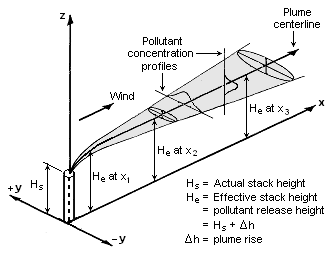
\includegraphics{gaussian-plume-schematic}
  \caption{Gaussian Plume Schematic, courtesy of English Wikipedia \cite{mbeychok_visualization_2007}. Note the differning notation from the schematic, where $x_1 = x$, $x_2 = y$ and $x_3 = z$. The numbered $x$ locations are different locations in the streamwise direction.}
  \label{fig:plume-schematic}
\end{wrapfigure}

The first bracketed term in the GPM \eqnref{eq:gpm} is the concentration of the pollutant per cross sectional area (with units mass per length). The second and third bracketed terms in \eqnref{eq:gpm} are the influence of the distribution in the transverse and vertical directions, respecitvely. The third term can be modified to model the effect of an inversion aloft or the reflection of the ground below by adding additional Gaussian terms, which mimic the effect of additional point sources in unphysical locations (e.g., $H$ meters below the ground) \cite{cimorelli_aermod_2005}. The influence of the distance in the downwind direction is to increase the variances $\sigma_2^2$ and $\sigma_3^2$ \eqnref{eq:gpm-variances} thereby diffusing the pollutant across an increasingly larger cross section. 

The GPM satisfies a few criteria which make it useful as a model. Firstly, the results of the model are generally consistent with observation \cite{sinha_application_2025, cimorelli_aermod_2005, kawka_downscaling_2023, lotrecchiano_pollution_2020, salih_air_2025}. Second, the model can be calculated explicitly, requiring very few computational resources. Finally, the GPM observes continuity. To demonstrate this, integrate \eqnref{eq:gpm} in the cross-sectional direction

\begin{equation} \label{eq:gpm-integral}
  \int_{-\infty}^\infty \int_{-\infty}^\infty C \,  dx_2 dx_3 = \frac{J_0}{U_0} \int_{-\infty}^\infty \int_{-\infty}^\infty \left[ \frac{1}{\sigma_2 \sqrt{2 \pi}} \exp \left( \frac{-x_2^2}{2 \sigma_2^2} \right) \right] \left[ \frac{1}{\sigma_3 \sqrt{2 \pi}} \exp \left( \frac{- (x_3 - H)^2}{2 \sigma_3^2} \right) \right] \, dx_2 dx_3 = \frac{J_0}{U_0}
\end{equation}

which follows from the standard result of the integration of a Gaussian function.

The first conceptual challenge of the GPM that follows immediately from \eqnref{eq:gpm-integral} is that nonzero concentrations of the pollutant species are calculated at an infinite distance from the point-source. Granted, most of the mass in any Gaussian distribution is within a few standard deviations of the mean; however, the fact that points a significant distance away contribute mass to the model is not physical.

The second challenge is that the GPM \X

\section{Methods}


\subsection{Dataset}

The data set (TURB-Smoke \cite{biferale_turb-smoke_2026}) is a direct numerical simulation (DNS) of millions of Lagrangian particles in an incompressible turbulent flow. In particular, a DNS of the three-dimensional Navier-Stokes equations was used to advect neutrally bouyant, nonreacting smoke particles seeded from one of five point sources.

The particles are then counted on a course-grained grid to obtain a concentration field. The concentration fields of all five point sources are distinct; however, for the purposes of this analysis, all five point sources were assumed to be colocated on the course grained mesh and the concentration fields of the five point sources were consequently summed.

The data set contains simulation runs with several different mean wind speeds ($U_0$). The mean wind speeds are provided as ratios to the root mean square speed, $U_{rms}$. The different values of these ratios are $U_0/U_{rms} = \{ 0, 1.03, 2.05, 4.11, 6.16 \}$. Note that for $U_0 / U_{rms} = 0$, the data model homogenous isotropic turbulence. For this analysis, we use $U_0/U_{rms} = 2.05$.

\fix{For the future submittal, I will include the different ratios as well, and create a comparison of the model performance for all of them. For this analysis I only have 2.05 because the website to download the data has been down for a month or so now. I am in contact with the corresponding author to try and get more data; however, generating the additional figures/analyses is comparatively simple once data arrives}.

\subsection{Parameter Choice}

\fix{Here, describe the choice of parameters against which the GPM was evaluated}.

\subsection{Statistics}

\fix{Here, develop analytically what the statistics of the GPM should look like.}

\subsection{Turbulent Model}

\fix{Here, develop analytically what the transport of the GPM should look like.}

\section{Results}

\fix{compare GPM to data, and better model}

\section{Discussion}

\section{Code and Data Availability}


% ----------------------------------------------------
% ------------------- bibliography -------------------
% ----------------------------------------------------

\bibliography{refs}
\bibliographystyle{aiaa}

\end{document}
